\documentclass[border=5mm]{standalone}
\usepackage{tikz}
\usepackage{amsmath}  % This provides \boldsymbol

\begin{document}

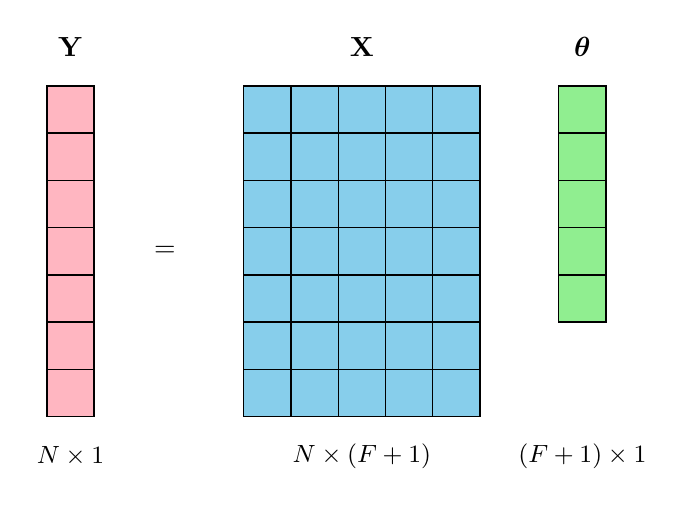
\begin{tikzpicture}
    % Define custom colors
    \definecolor{pinkcell}{HTML}{FFB6C1}
    \definecolor{bluecell}{HTML}{87CEEB}  
    \definecolor{greencell}{HTML}{90EE90}

    % Vector Y (pink) - 7x1
    \foreach \i in {0,1,2,3,4,5,6} {
        \draw[fill=pinkcell, draw=black, line width=0.5pt] 
            (0, -\i*0.6) rectangle (0.6, -\i*0.6-0.6);
    }
    
    % Equals sign
    \node at (1.5, -2.1) {$=$};

    % Matrix X (blue) - 7x5
    \foreach \i in {0,1,2,3,4,5,6} {
        \foreach \j in {0,1,2,3,4} {
            \draw[fill=bluecell, draw=black, line width=0.5pt] 
                (2.5+\j*0.6, -\i*0.6) rectangle (2.5+\j*0.6+0.6, -\i*0.6-0.6);
        }
    }

    % Vector theta (green) - 5x1
    \foreach \i in {0,1,2,3,4} {
        \draw[fill=greencell, draw=black, line width=0.5pt] 
            (6.5, -\i*0.6) rectangle (7.1, -\i*0.6-0.6);
    }

    % Labels above
    \node at (0.3, 0.5) {$\mathbf{Y}$};
    \node at (4, 0.5) {$\mathbf{X}$};
    \node at (6.8, 0.5) {$\boldsymbol{\theta}$};

    % Dimension labels below
    \node at (0.3, -4.7) {\small $N \times 1$};
    \node at (4, -4.7) {\small $N \times (F+1)$};
    \node at (6.8, -4.7) {\small $(F+1) \times 1$};

\end{tikzpicture}

\end{document}